\documentclass{article}
\usepackage[
backend=biber,
style=alphabetic,
]{biblatex}
\addbibresource{rcheruiyotrefs.bib} %Imports bibliography file
\usepackage[utf8]{inputenc}
\usepackage{graphicx}
\usepackage{float}
\graphicspath{ {./images/} }
\usepackage{multicol}
\usepackage{setspace}

\setlength{\columnsep}{1cm}

\title{Brief Intro About Me}

\author{Raymond Cheruiyot (Rono), PhD in Security}
\date{August 2022}

\begin{document}

\maketitle

\begin{multicols}{2}

\section{My goals in this program}
Hi, I am starting my first year in the PhD Security program being advised by Dr. Chang. I am still working on a more formal topic for my research with him. My background is on data science and as I look at cybersecurity I see a number of opportunities to utilize data science techniques to solve some of the cybersecurity challenges. My research interests lean mostly towards optimal dimensionality reduction in feature engineering, use of neural networks in blockchain security and machine learning application to network traffic monitoring. In order to be equipped with the skills and knowledge required to do a competitive research work, I have enrolled in the course CS 6000, Computer Science Research. 

My expectation is that this course will improve my ability to learn and enable me to carry out efficient research. I have an intention to share the outcome of my research work and I believe CS 6000 will help me with the know how of how to publish the work as well as benefit from the work already done by others. My goals is to be able to: critically review research reports and to synthesize a body of literature; write research reports and to present findings; draw conclusions from the research and to assess the generalizability of study results; and write a research proposal and dissertation suitable and meeting requirements for submission to a research evaluation committee.



Outside classwork, you will find me taking hikes or playing a game of chess. I do like travelling and nature walk when travelling is constraining. Occasionally I do jump onto a bike and cycle around.

\end{multicols}

\section{Figures}
\begin{figure}[H]
 \centering
 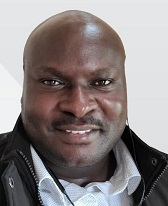
\includegraphics[width = .5\textwidth]{images/myImage2.jpg}
 \caption{A recent photo of me}
 \label{fig:float}
\end{figure}
\begin{figure}[H]
 \centering
  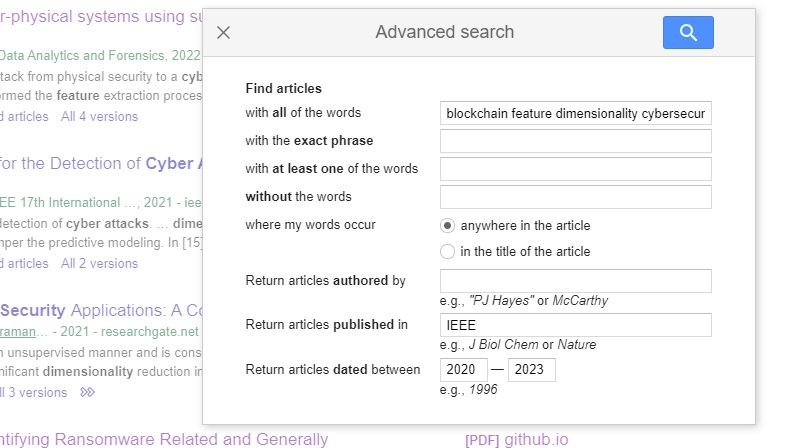
\includegraphics{images/myImage4.jpg}
 \caption{Using advanced search in google scholar}
 \label{fig:2}
\end{figure}

\begin{figure}[H]
 \centering
  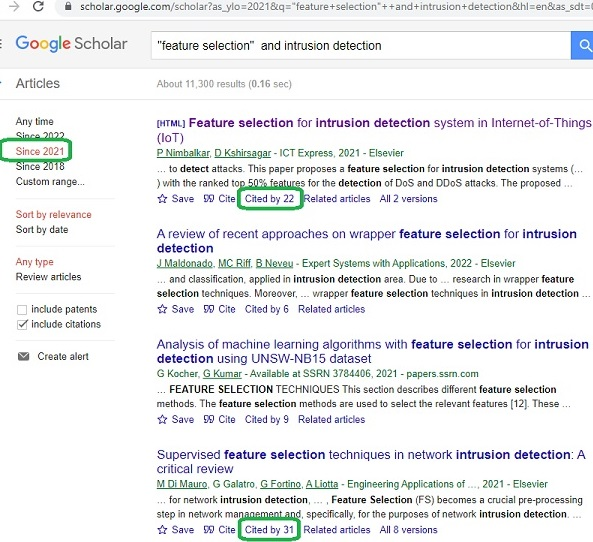
\includegraphics{images/myImage3.jpg}
 \caption{I searched in google scholar the key words 'feature selection and intrusion detection. Using the recency of the articles and the number of citations, I picked papers related to my area of interest}
 \label{fig:2}
\end{figure}

\section{About my research}

Ethereum is a blockchain platform where users can transact cryptocurrency as well as build and deploy decentralized applications using smart contracts, however detecting such activities such as ponzi-scheme, tax evasion by transacting in cryptocurrency, using pseudo-anonymous accounts for receiving ransom payment, consolidation of funds accumulated under multiple identities etc. should be monitored and detected in order to keep legitimate users safe on the platform. It can be demonstrated that supervised machine learning based anomaly detection can be used to to solve the challenges being experienced \cite{kumar2020detecting}.

Crypto-assets and blockchain technologies hold the promise of providing more secure systems for managing public and private data, enhancing public trust in data collection, and increasing the efficiency of social impact finance transactions. However, to date, blockchain technologies have struggled to deliver on these promises. Specifically, cybersecurity threats to blockchain technologies are accelerating and becoming more impactful over time. This generates growing risk toward the use of the blockchain technologies in social impact finance services provision \cite{gurdgiev2021informational}.

Research indicates that machine learning tools can be used to solve any attack detection problem which can remedy model selection issues \cite{berghout2022machine}.

Deep learning has a better effect on some aspects of cyber security and should be considered as the first option.\cite{li2021deep}.

Cybersecurity data science is a very emerging field that protects systems, networks, and data from digital attacks. With the increase in the scale of the Internet and the evolution of cyber attacks, developing novel cybersecurity tools has become important, particularly for Internet of things (IoT) networks. Deep learning (DL) approaches for cybersecurity challenges do exist.\cite{podder2021artificial}.
\par
 \doublespacing
The well known Pythagorean theorem \par \(x^2 + y^2 = z^2\) \par and the equation \par
 \doublespacing
\begin{equation*} \sum _{t=1}^{T}\Vert {\hat{H}_t-H_t}\Vert +\beta \Vert W\Vert _2 \tag{11} \end{equation*}

where hat{H}_t, Ht  is the input of network that we can reconstruct, and ∥W∥2 is the l2-norm of network weights.

\nocite{jain2004introduction}
\nocite{yu2003ga}
\nocite{roy2018protection}
\nocite{zhang2021research}
\nocite{lecun2015deep}
\nocite{bai2021know}
\nocite{yu2021information}
\nocite{xu2018industry}
\nocite{culot2019addressing}
\nocite{meneghello2019iot}
\nocite{wang2019blockchain}
\nocite{falco2018iiot}
\nocite{pan2015classification}
\nocite{zhang2003data}
\nocite{demertzis2018next}
\nocite{hao2016mining}
\nocite{zhao2019blockchain}
\nocite{gurdgiev2021informational}
\nocite{jain2004introduction}
\nocite{podder2021artificial}

\medskip

\section{Tools used}
Online Latex
This tool is a document formatting program and new to me and I interacted with it through overleaf. I am still learning how to use it properly. The challenges of using it is that it has no spell checking, difficult to learn and use and  needs structured way of doing things. However once one is familiar with the tool it seems it's a good tool for organizing papers. I also used google scholar to search for references. 


\section{Questions}
Please place your questions here:

Q: How etherum is different from bitcoin? which encryption algorithms used in both cryptocurrency?

Hi,
BTC and ETH are both digital currencies, but the primary purpose of ether is not to establish itself as an alternative monetary system but to facilitate and monetize the operation of the smart contracts. 
No, Bitcoin does not use encryption. It's called “cryptocurrency” because its digital signature algorithm uses the same mathematical techniques used for a type of encryption based on elliptic curves. Bitcoin uses the Elliptic Curve Digital Signature Algorithm (ECDSA) with the elliptic curve secp256k1, not encryption

\subsection{Question 1 (from Hassan)}
Hi Rono, Where you usually go for hiking?
Hi Hassan. I mostly do the Garden Of The Gods Park, Palmer Park, Bear Creek Dog Park and Manitou Incline. The last one is challenging though!

\printbibliography
\end{document}
